\chapter{Webpage Classification}\label{chapter:clf}
This chapter will give a detailed explanation on the agent \textbf{Filter} which responsible for the web page judgement, and show the experiments results.

Judge that weather the webpage sent from crawlers is a target page is the first key part of this whole pipeline. We will combine the techniques of visual analytics and webpage automatic classification to implement a more efficient and more accurate webpage filter as shown in Figure \ref{fig:fc:filter}

\begin{figure}[htb!]
	\centering
	\includegraphics[page=6,width=\textwidth]{images/diagrams.pdf}
	\caption{Flow Chart for Filter}\label{fig:fc:filter}
\end{figure}


For convenience, we use the following numerical digits to represent the classification of webpages. Meanwhile, we define three colours correspondingly. This helps the users clearly recognise the different classifications in visualisation system.
\begin{table}[htb!]
\small
\centering
\vspace{-1.5em}
\caption{Integer Presentation for Classification}
\begin{tabular}{@{}cp{0.3\textwidth}p{0.4\textwidth}c@{}}
\toprule
  \textbf{Integer}   
& \textbf{Class}
& \textbf{Description} 
& \textbf{Color}\\ 
	\midrule -1
	& Non-Target Page
	& Tis page contains no seminar announcement information
	& \colorbox{c_non}{\color{white}-1} \\
	\midrule 0
	& Default	& hasn't been decided. This class does not exist in the data set
	& N/A\\
	\midrule 1
	& Single Target Page 
	& This page contains exact one seminar announcement information
	& \colorbox{c_sin}{\color{white}\ 1}\\
	\midrule 2
	& Multiple Targets Page
	& This page contains more than one seminar announcement information
	& \colorbox{c_mul}{\color{white}\ 2}\\
	\bottomrule
\end{tabular}
\vspace{-2.5em}
\end{table}

\section{Feature Extract}
\vspace{-0.5em}
When \textbf{Filter} receives command \code{new} from crawler(i.e. when a new item arrives at \textbf{Filter}), it will load the item from the database and file system(i.e. \textbf{Filter}'s inbox) according to the \code{item_id} in the received message. Then, if the classification decision of this item has not been decided, we will use our ontology-based Feature Extractor to extract the feature vector of this webpage item. It will extract every required feature and then combine them together\cite{pasupat2014zero}.

There are several critical reasons why we need feature extraction. Feature extraction uses the given feature space to turn the content of a webpage into a feature vector so that we will be able to process data\cite{devi2008generating}. Meanwhile, the vectors extracted by Feature Extractor can show the characteristics of the original webpage to a great extent and thus make the following classification meaningful\cite{FeatureSelection2011,pasupat2014zero}.

With the consideration that our research target is HTML and even HTTP response, we define the following three types of feature. These features can be defined according to common sense or the suggestions from the human experts in the target topic. Some of them can be regarded as the index of the possibility that a web page is target; these are positive features($+$), while the others are negative features($-$). The features are all defined manually based on a large number of surveys conducted by ourselves.

\subsection{Literal Features}
Literal Features are the features only extracted from the text in the HTML.
\begin{table}[htb!]
\small
\centering
\caption{Candidate Literal Features}
\vspace{-0.5em}
\label{tab:ca_feature:literal}
\resizebox{\textwidth}{!}{%
\begin{tabular}{@{}p{0.1\textwidth}p{0.35\textwidth}p{0.4\textwidth}c@{}}
\toprule
\textbf{ID} & \textbf{Feature} & \textbf{Description} & \textbf{Property} \\ \midrule
$fl_{0}$ 
	& number of seminar indicators 
	& count the number of synonym words which can be a indicator for seminar, e.g. \textit{seminar}, \textit{talk}
	& + \\ \midrule
$fl_{1}$ 
	& number of topic indicators 
	& count the number of synonym words which can be a indicator for topic, e.g. \textit{topic:}, \textit{title:}
	& + \\ \midrule
$fl_{2}$ 
	& number of speaker indicators 
	& count the number of indicator words for speaker, e.g. \textit{speaker:}, \textit{instructor:}, \textit{who:}
	& + \\ \midrule
$fl_{3}$ 
	& number of location indicators 
	& count the number of indicator words for location, e.g. \textit{location:}, \textit{venue:}, \textit{place:}
	& + \\ \midrule
$fl_{4}$ 
	& number of date and time indicators 
	& count the number of indicator words for date and time, e.g. \textit{date:}, \textit{time:}, \textit{start from:}
	& + \\ \midrule
$fl_{5}$ 
	& number of abstract indicators 
	& count the number of indicator words for abstract, e.g. \textit{introduction:}, \textit{abstract:}, \textit{start from:}
	& + \\ \midrule
$fl_{6}$ 
	& number of speaker entities 
	& count the number of entity for speaker, e.g. \textit{Dr.}, \textit{Professor:}, \textit{Mr.}
	& + \\ \midrule
$fl_{7}$ 
	& number of location entities 
	& count the number of entity for location, e.g. \textit{room}, \textit{theatre}, \textit{building}
	& + \\ \midrule
$fl_{8}$ 
	& number of date and time entities
	& count the number of entity for date and time, e.g. \textit{13:20}, \textit{2015-01-03}
	& + \\ \midrule
$fl_{9}$ 
	& difference between the number of location and speaker entities
	& normally, the number of location and speaker entity are closed in a seminar announcement page
	& + \\ \midrule
$fl_{10}$ 
	& ratio of the number of location and date/time entities
	& 
	& + \\ \midrule
$fl_{11}$ 
	& number of `tbc'
	& count the number of `tbc' or `tba' in the page
	& + \\ \bottomrule
\end{tabular}
}
\end{table}


\subsection{Structural Feature}
Due to that HTML documents are structural, we define the following structural feature with making use of DOM tree of HTML.

\begin{table}[htb!]
\small
\centering
\caption{Candidate Structural Features}
\label{tab:ca_feature:struct}
\begin{tabular}{@{}p{0.1\textwidth}p{0.3\textwidth}p{0.4\textwidth}c@{}}
\toprule
\textbf{ID} & \textbf{Feature} & \textbf{Description} & \textbf{Property} \\ \midrule
$fs_{0}$ 
	& number of img tag 
	& this feature indicates the number of the images in the webpage, a seminar announcement page might not have too many images.
	& - \\ \midrule
$fs_{1}$ 
	& number of table tag 
	& this feature indicates the number of the tables in the webpage.
	& + \\ \bottomrule
\end{tabular}
\end{table}


\subsection{Other Feature}
As a matter of fact, the target research entities in this project are HTTP responses. Therefore, we need to consider other factors instead of the html entity. We call this kind of factors ``special features'', which may include: 

\begin{table}[htb!]
\small
\centering
\caption{Candidate Other Features}
\label{tab:ca_feature:other}
\begin{tabular}{@{}p{0.1\textwidth}p{0.3\textwidth}p{0.4\textwidth}c@{}}
\toprule
\textbf{ID} & \textbf{Feature} & \textbf{Description} & \textbf{Property} \\ \midrule
$fo_{0}$ 
	& number of seminar indicator in URL 
	& whether indicator words for seminar exist in the URL. e.g. \textit{seminar}, \textit{talk}
	& + \\ \midrule
$fo_{1}$ 
	& number of negative indicator in URL 
	& some words in URL may indicate to some negative entity. e.g. \textit{blog}, \textit{article}, \textit{document}
	& - \\ \bottomrule
\end{tabular}
\end{table}

\subsection{Feature Extraction Ontology}
In order to implement a feature extraction ontology which can cover all above features flexibly, we give a formal definition on the feature extract rule: 
\begin{defn}
A feature extract rule is a tuple $\langle S, \mathcal{R}, P, W \rangle$, the result of this feature extract rule $f=\langle S, \mathcal{R}, P, W \rangle$ for a HTTP response $X$
\begin{eqnarray}
	\phi_f(X) &=& \phi_{\langle S, \mathcal{R}, P, W \rangle}(X)\\
	&=& W \times \operatorname{P}\limits_{r \in \mathcal{R}}\lbrack \# \operatorname{Match}_r(\operatorname{Select}_S(H))\rbrack
\end{eqnarray}
where:
\begin{itemize}
	\item $S$ is a scope selector, it will pick a specific part of a HTTP response, it can be:(default is html)
		\begin{itemize}
			\item html: the whole HTML document
			\item text: the text in HTML document, it will ignore all tags in the HTML.
			\item tag: the HTML tags in HTML document, it will ignore all text in the HTML.
			\item title: text in \texttt{<title>} tag
			\item keywords: content of tag \texttt{<meta name='keywords'>}\\
			this filed normally is used for SEO(Search Engine Optimisation), sometimes webpage author will provide abstract keywords of the current page in this field. 
			\item description: content of tag \texttt{<meta name='description'>}\\
			this filed normally is used for SEO(Search Engine Optimisation), sometimes webpage author will provide abstract description of the current page in this field. 
			\item url: the URL of the HTTP response. 
		\end{itemize}
	\item $\mathcal{R}$ is a set of regular expressions, which used to match the output of the selector 
	\item $P$ is a policy, used to be adapted to the count of each matches, the policy could be:
		\begin{center}
			sum $\vert$ max $\vert$ min $\vert$ avg $\vert$ prod $\vert$ div $\vert$ exist
		\end{center}
	\item $W$ is the weight of this feature, used to scale the value of this feature. (default is 1)
\end{itemize}
\end{defn}

So the feature extraction function $\phi$ is shown in Figure \ref{fig:feature_extraction}. For a HTTP response, a feature extract function will:
\begin{enumerate}
	\item use $S$ to select the target scope of the HTTP response
	\item for each regular expression $r \in \mathcal{R} $, match function will be applied on the selected scope, it will output a array including the number of match elements for each $r$
	\item a policy $P$ then will applied on this array, let the result multiply a weight $W$ to get the feature value.
\end{enumerate} 

\begin{figure}[htb]
	\centering
	\includegraphics[page=8,width=\textwidth]{images/diagrams.pdf}
	\caption{Feature Extraction}\label{fig:feature_extraction}
\end{figure}

In order to make the feature extraction rule understandable for the system, we give a ontology representation for feature extraction rule in XML format. Here, we use $fl_{10}$ as an example: Code \ref{code:onto_fer}.
\vspace{1em}
\lstinputlisting[language=xml,label={code:onto_fer},caption=Ontology Representation for Feature Extraction Rule]{./src/onto_feature.xml}

It could be seen that even relatively complicated features, such as $fl_10$, have a clear structure and logic in our ontology. We have two list nodes here. They will load two external files separately, which are regular expression list forms of location and datetime entities. For the entire feature, we apply \texttt{div}(division) policy so that the ratio of the two kinds of entities could be obtained. $S$ and $W$ are not given, therefore we use their default values.

In order to get a feature vector in various dimensions, we introduce the concept of feature space:
\begin{defn}
	Feature space $F$ is a list contains all feature extraction rules to conduct feature extraction.	So the element in feature vector $\upsilon$ of a HTTP response under a feature space $F=\{f_1, f_2, \dots, f_n\}$:
	\begin{equation}
		\upsilon_i = \phi_{F_i}(X) \mbox{\space for $i \in [1,n]$}
	\end{equation}
\end{defn}

In ontology representation, its\footnote{The XML Schema for feature space is given in the Appendix \ref{apdx:fe_onto} }:

\lstinputlisting[language=xml,caption=Ontology Representation for Feature Space]{./src/onto_featurespace.xml}

It could be seen that during the process of feature extraction, selector $S$ used to choose the parts that are often similar to HTTP response. For the purpose of ensuring high efficiency, we implemented a cache map. Different parts of HTTP response will be loaded in a lazy mode and then stored into this cache map in order to improve the efficiency during the feature extraction.

\section{Feature Selection}
In the field of statistics and machine learning, feature selection is a core process in model construction. It is the approach of selecting a subset of relevant features. It simplifies the models so that it is easier for user to interpret. Meanwhile, it shortens the training time and enhances generalisation by reducing overfitting\cite{james2013introduction}.

\begin{figure}[htbp]
	\centering
	\includegraphics[page=5,width=\textwidth]{images/picture.pdf}
	\caption{Parallels Coordinate}\label{fig:feature_selection:pd}
\end{figure}

Due to the features are defined by human experts, there might be some redundant features in the candidate features set. For instant, some features may not have strong correlation to the classification result, even some features have strong correlation with each others. These redundant features have no positive influence on classifier training, but increase the training time, so we need feature selection technique to reduce the dimension.

In addition, our classifier model is decision trees. When the number of features becomes large, the decision tree inclines to overfit the data. It is crucial that we get the appropriate ratio of samples to the number of features in that a tree with few samples in high dimensional space is more possible to overfit. 

Now, we are going to do selection among the candidate features we listed above. Usually, calculating \textbf{Pearson's product moment coefficient} among these features and label is a fine choice\cite{lee1988thirteen}. Nevertheless, we will use a more intuitive way for humans to make decisions directly in this project, which is making use of visualisation to assist the feature selection.

At beginning, we use a feature space\footnote{This feature space is given in the Appendix \ref{apdx:fe_onto} } that contains all the 16 candidate features above to do feature extract on \textbf{OXSEM} dataset. Then, draw a parallel coordinate which shows the correlation among all the candidate features and their labels clearly (see the Figure \ref{fig:feature_selection:pd}).

The first column is the classification label of the data in our \textbf{OXSEM} dataset. After this, it lists all 16 candidate feature, where each line which connects different axes is a piece of data. We use the colour we defined before to mark the cluster of the three different kinds of data. And because of the space limitation, we will give the magnified charts in the appendix.

\begin{figure}[htb!]
	\centering
	\includegraphics[page=11,width=\textwidth]{images/diagrams.pdf}
	\caption{Parallels Coordinate}\label{fig:feature_selection:pd_pattern}
\end{figure}
\begin{figure}[htb!]
	\centering
	\includegraphics[page=7,width=\textwidth]{images/picture.pdf}
	\caption{Pattern Example in Parallels Corrdinate}\label{fig:feature_selection:pd_exp}
\end{figure}

By adjusting relation with label during the adjusting process. Basically, we are looking for features according to the following policy.
\begin{enumerate}
  \item We prefer the distribution in Figure \ref{fig:feature_selection:pd_pattern}($a$) that the red lines(single target pages) are much more aggregate than the yellow lines(multiple targets pages). Thus, that feature is more distinct on red class. A typical example of this kind of feature is the ($fs_0$) in Figure \ref{fig:feature_selection:pd_exp}(1). The red and yellow lines are apparently more aggregate than the grey lines. However, there is a single yellow line above the others; we consider it as noise.
  \item We also prefer the distribution in Figure \ref{fig:feature_selection:pd_pattern}($b$) in that the two different class of lines are separated clearly. Therefore, the two has a relatively high discrimination. The examples are $fo_0$ in Figure \ref{fig:feature_selection:pd_exp}(2) and $fl_9$ in Figure \ref{fig:feature_selection:pd_exp}(3). The red lines and grey lines are dispart with each other.
  \item We do not want a distribution like Figure \ref{fig:feature_selection:pd_pattern}($c$). The lines are disorderly and unsystematic, makes it undistinguishable and can hardly get any useful information from the graph. The example is $fs_1$ in Figure \ref{fig:feature_selection:pd_exp}(4). The order of the lines are in a mass.
\end{enumerate}

By changing the order of the axis, we could discover two other patterns: ($d$) and ($e$) (see Figure \ref{fig:feature_selection:pd_pattern}).

In ($d$) and ($e$), the same kind of lines are all parallel. We only need one of ($d$) and ($e$). Because these two features share a high correlation. Keeping one of them is enough, while the other one is redundant. Typical instances are $fl_{10}$ and $fl_7$ in Figure \ref{fig:feature_selection:pd_exp}(5).

Combined with the analysis of the above, we finally decide to apply the following 12 features. and we create a featurespace $F^\star $ including the following features, $F^\star $ will be used to extract feature from all the webpage.

$$F^\star = \{ fl_0,fl_1,fl_2,fl_3,fl_4,fl_5,fl_6,fl_8,fl_9,fs_0,fo_0,fo_1 \} $$


\section{Classification and Active Learning}
After obtaining the feature vector, the classification process is done with the help of a pre-defined decision tree generated by the training data. If so, define whether it is a single seminar page or a multiple seminar page. Furthermore, it will not only give the decision result, but also the probability of the certainty (i.e. confidence value) to this result. Therefore, if a result has a confidence higher than the pre-defined threshold, it will give a doubtless decision (although maybe still not has 100\% correctness). 

\subsection{Decision Tree}
For classification and regression, Decision Tree is an ideal learning method which is non-parametric and supervised. The aim of this method is creating a model to predict the value of a target variable by simple decision rules learnt from the features of data\cite{breiman1984classification,quinlan2014c4,friedman2001elements}. 

Once generated by fitting the training data, the decision tree will keep updating itself automatically based on the decisions corrected by human experts(users) or the returned correction from \textbf{Extractor}.

In our implementation, the classification decision tree is implemented by using the CART (Classification and Regression Trees) algorithm\cite{quinlan2014c4,friedman2001elements} with a parameter $\theta$ which contains:
\begin{equation}
	\theta : \left\{
		\begin{aligned}
		\theta_D & :  \mbox{maximum depth of the tree allowed} \\
		\theta_M & :  \mbox{minimum number of sample in a node to split} \\
		\theta_C & :  \mbox{classification criterion function}
		\end{aligned}
	\right.
\end{equation}
For a training dataset $(\bv{x},\bv{y})$, where $\bv{x} \in R^n$ is the feature vectors of the webpage, $\bv{y}$ is the label vector. decision tree will partition the dataset recursively at each node of the tree according to specific feature.

We firstly define a split function as following:
\begin{equation}
	\tau = (f,t_{f})
\end{equation}

where $f$ is a specific feature, $t_{f}$ is the threshold on feature $f$. Then, if we use $T_k$ to denote the dataset contains the subtree rooted as node $k$, it would be split two two subtree according to a specific split function $\tau_k$. the left subtree dataset $L_k(\tau_k)$ and right subtree dataset $R_k(\tau_k)$ are:

\begin{eqnarray}
	L_k(\tau_k) &=& \{ (\bv{x},\bv{y}) \vert (\bv{x},\bv{y}) \in T_k, \bv{x}_f <= t_{f,k} \mbox{where } \tau_k = (f,t_{f,k}) \}\\
	R_k(\tau_k) &=& T_k \backslash L_k(\tau_k)
\end{eqnarray}

Then we can calculate the impurity at node $k$ by:
\begin{equation}
	\Gamma(T_k,\tau_k) = \frac{\vert L_k(\tau_k) \vert \cdot \theta_C(L_k(\tau_k)) + \vert R_k(\tau_k) \vert \cdot \theta_C(R_k(\tau_k)) }{\vert T_{k} \vert}
\end{equation}



The target function of the classification is find the best $\tau_k$ (best feature and threshold to use) recursively 
\begin{equation}
	\tau_k^\star = \arg\min_{\tau_k}\Gamma(T_k,\tau_k)
\end{equation}
until one of the two constraints reached:
\begin{eqnarray}
	\operatorname{depth}(k) = \theta_D\\
	\vert T_{k} \vert < \theta_M
\end{eqnarray}

we also define proportion of these for three classes (-1,1,2) of observations in node $k$

\begin{equation}
	p_{k,l} = \frac{1}{\vert T_k \vert}\sum\limits_{\bv{x}_i\in T_k}I(y_i = l) \mbox{ for $l \in \{-1,1,2\}$} 
\end{equation}
For classification criteria function $\theta_C$, we have three options:

\textbf{Gini:}
\begin{equation}
	\theta_C = \sum\limits_l p_{k,l}(1-p_{k,l}) \mbox{ for $l \in \{-1,1,2\}$}
\end{equation}

\textbf{Cross\text{-}Entropy:}
\begin{equation}
	\theta_C = \sum\limits_l p_{k,l}\log(p_{k,l}) \mbox{ for $l \in \{-1,1,2\}$}
\end{equation}

\textbf{Misclassification:}
\begin{equation}
	\theta_C = \sum\limits_l 1-\max(p_{k,l}) \mbox{ for $l \in \{-1,1,2\}$}
\end{equation}

Overall, the training process of the decision tree is keep selecting the most distinguishable feature and threshold for decision making according to the target function.

In order to prevent the decision tree from over-complex and further cause overfitting, we are going to solve this problem in the following aspect instead of the feature selection we have already done before.

\begin{enumerate}
	\item  $\theta_D$: because of the number of sample data, the decision tree will keep adding new levels to grow\cite{breiman1984classification}. By setting a proper $\theta_D$, the maximum	depth(i.e. complexity) of the decision tree could be under control, and thus avoid overfitting.
	\item $\theta_M$: a very tiny $\theta_M$ may cause the decision tree be too meticulous and thereby overfitting\cite{quinlan2014c4}. However, an overlarge $\theta_M$ will prevent the tree from learning the data. Hence, an appropriate $\theta_M$ is able to ensure that leaf nodes contain samples of different labels other than continue to split using new features. This also helps with preventing overfitting of the decision tree.
\end{enumerate}

Because of the existence of $\theta_M$, our leaf nodes might take on data samples of different labels. Consequently, we define the confidence value.

\begin{defn}
	If an entity $\bv{x}_0$ is classified as $l_0$ through the leaf node $T_0$ of the decision tree, the confidence value is defined as:
	\begin{eqnarray}
		\eta &=& \Pr(l=l_0) \mbox{ for all $(\bv{x},y) \in T_0$}\\
		     &=& \frac{ \vert T_0^\prime  \vert }{\vert T_0 \vert} \mbox{ where $T_0^\prime = \{ (\bv{x},y) \vert (\bv{x},y)\in T_0, y = l_0 \}$}
	\end{eqnarray}
\end{defn}

A confidence value will be given together with a decision. If the confidence is above the \texttt{CONFIDENCE\_THRESHOLD} (this was set by the human expert as a part of the system configuration), then make the decision directly. The decision will be saved to the database and passed to Extractor. Otherwise, when the confidence is below the \texttt{CONFIDENCE\_THRESHOLD}, this webpage will be labelled as `unknown' and put back into the filter list for human experts to decide.

\subsection{Human Interaction and Active Learning}
\begin{figure}[htb!]
	\centering
	\includegraphics[page=6,width=0.9\textwidth]{images/picture.pdf}
	\caption{Filter: Human Interaction}\label{fig:filter:hi}
\end{figure}
As we stated above, if the confidence value of a decision to a item did not meet the \texttt{CONFIDENCE\_THRESHOLD}, this item will be put in a filter list which will show in our web interface. Users can visually intervene through visual analytics and conduct fast correction in the filter list webpage after a simple short training. We will keep updating the decision tree classfier. This is an active learning process, which will ultimately make the classification result be more accurate.

The Figure \ref{fig:filter:hi} has some visual and interaction elements:
\begin{enumerate}
	\item \textbf{Entity Information}\\
	It provides the user with the basic information of this record, including ID(in system), title and URL address so that user could do a fast judgement from the title and URL.
	\item \textbf{Decision Indicator}\\
	This is the decision made automatically by the classifier inside the \textbf{Filter}. The background colour represents the decision of the \textbf{Filter}. The number represents the confidence value we mentioned before. This indicator could give machine learning assistance for users to do quick decision making. The area of the coloured lines also represents the confidence value, which is more visual and intuitive than numbers.
	\item \textbf{Quick Correct Button}\\
	User can do fast correction manually by clicking on three buttons: N(stand for Non-Target Page), S(stand for Single-Target Page), and M(stand for Multiple-Target Page).
	\item \textbf{Modal Preview}\\
	If user still cannot make decision by the two methods above, he can click the URL button in (1) and view the local webpage cache in the modal window. Observing the actual webpage could help the user make decisions in a short time.
\end{enumerate}

The user correction data will be recorded by \textbf{Filter}. \textbf{Filter} uses all the sample to re-train the decision tree. However, it will not do so until it receives the \texttt{refresh} command(user can do this by clicking the button on the left). The reason we do not do proactive re-train is that when the number of corrections is very small, it does not have a great influence on the decision tree, but cause a waste of time instead. So we use mini-batch update. Meanwhile, a correction made by a large number of new samples will cause the sample number of training data for decision tree quickly increasing and therefore cause overfitting. Whereas the methods we proposed before are able to avoid overfitting effectively.

\section{Experiment}

\subsection{Setting and Measure}
We take 1300 pieces of record among the entire OXSEM-Dataset as the dataset of the experiment. We use \textbf{Recall}, \textbf{Precision} and \textbf{F-measure} as the evaluation criteria for this classification problem.

\begin{defn}
For a test dataset $T$ with the assumption:

\begin{eqnarray}
	T_+ &=& \{(\bv{x}, y) \in T \vert y\in \{1,2\} \}\\
	T_- &=& \{(\bv{x}, y) \in T \vert y=-1\}
\end{eqnarray}

And after the automatic classification, the filter labelled the dataset as $T^\prime$ and:
\begin{eqnarray}
	T^\prime_+ &=& \{(\bv{x}, y^\prime) \in T^\prime \vert y^\prime\in \{1,2\} \}\\
	T^\prime_- &=& \{(\bv{x}, y^\prime) \in T^\prime \vert y^\prime=-1\}
\end{eqnarray}
Then we have $recall$, $precision$ and $f-measure$ as following:
\begin{eqnarray}
	precision &=& \frac{T^\prime_+ \cap T_+ }{T^\prime} \\
	recall &=& \frac{T^\prime_+ \cap T_+ }{T} \\
	f-measure &=& 2\times \frac{recall \times precision}{recall + precision} 
\end{eqnarray}
\end{defn}

Then, we have several parameters configurations to test our decision tree:
\begin{table}[htb!]
\small
\centering
\caption{Parameters Configurations for Decision Tree}
\label{tab:exp:para}
\begin{tabular}{@{}cccc@{}}
\toprule
\textbf{ID} & $\theta_D$ & $\theta_M$ & $\theta_C$ \\ \midrule
$\theta^1$ 
	& 6
	& 20
	& `gini' \\ \midrule
$\theta^2$ 
	& 6
	& 20
	& `cross-entropy' \\ \midrule
$\theta^3$ 
	& 12
	& 20
	& `gini'\\ \midrule
$\theta^4$ 
	& 4
	& 20
	& `gini'\\ \midrule
$\theta^5$ 
	& 8
	& 10
	& `gini'\\
	 \bottomrule
\end{tabular}
\end{table}

The choice of training set will have a huge impact on the test result. In order to prevent such influence, our experiment will do cross-validation. It is important that we do cross-validation in that we need to guard against testing hypotheses suggested by the data, which is usually called Type III errors\cite{kohavi1995study}. The necessity is more than ever when the further samples are costly, hazardous, or barely being collect.

@We split the data set into ten groups, each has 130 pieces of data with average distribution of None, Single and Multiple seminar announcement webpage. We use them to do \textbf{Stratified K-Fold Test} to ensure the reliability of the test. In k-fold cross-validation, the original sample is randomly divided into $k$ subsets with same size. In these k subsets, there are $k-1$ subsets are used as training dataset to train the model, the remaining one is regarded as test dataset to validate the trained model.\textbf{Stratified K-Fold Test}\cite{refaeilzadeh2009cross} requests the data for each class is averagely distributed in all $k$ folders. The train and test will repeated $k$(the number of folds) times with different training dataset and test dataset in the entire cross-validation process, with each of the $k$ subset used exactly once as the validation data. The final single estimation result is the average of $k$ results\cite{mclachlan2005analyzing}.

\subsection{Experiment Result and Analysis}
For this kind of project, considering our system design, we wish for a higher recall. Because compared with recall, we could make up precision to some degree by artificial intervention which assists manual correction. It could be seen that through the \textbf{Filter} we developed based on our designed ontology, a delightful recall and an encouraging precision have been achieved\footnote{However, we do not especially distinguish between Single Target Page and Multiple Targets Page}. With the help of visualisation and human interaction, this precision could be even higher. For these parameter configuration, the result of cross-validation shown as in Table \ref{tab:exp:result}

\begin{table}[htb!]
\centering
\caption{Test Result for Different Settings}
\label{tab:exp:result}
\textbf{$\theta^1$}
\vspace{1em}
\resizebox{\textwidth}{!}{%
\begin{tabular}{@{}llllllllllll@{}}
\toprule
-         & folder 0 & folder 1 & folder 2 & folder 3 & folder 4 & folder 5 & folder 6 & folder 7 & folder 8 & folder 9 & average \\ \midrule
precision & 89.13\%  & 79.25\%  & 64.91\%  & 96.77\%  & 96.77\%  & 100.00\% & 85.29\%  & 84.75\%  & 95.08\%  & 84.51\%  & 87.65\% \\
recall    & 68.33\%  & 70.00\%  & 61.67\%  & 100.00\% & 100.00\% & 95.00\%  & 96.67\%  & 83.33\%  & 96.67\%  & 100.00\% & 87.17\% \\
f-measure & 77.36\%  & 74.34\%  & 63.25\%  & 98.36\%  & 98.36\%  & 97.44\%  & 90.62\%  & 84.03\%  & 95.87\%  & 91.60\%  & 87.12\% \\ \bottomrule
\end{tabular}

}

\textbf{$\theta^2$}
\vspace{1em}
\resizebox{\textwidth}{!}{%
\begin{tabular}{@{}llllllllllll@{}}
\toprule
-         & folder 0 & folder 1 & folder 2 & folder 3 & folder 4 & folder 5 & folder 6 & folder 7 & folder 8 & folder 9 & average \\ \midrule
precision & 89.19\%  & 82.00\%  & 71.83\%  & 95.16\%  & 98.33\%  & 100.00\% & 85.71\%  & 87.10\%  & 90.91\%  & 87.50\%  & 88.77\% \\
recall    & 55.00\%  & 68.33\%  & 85.00\%  & 98.33\%  & 98.33\%  & 96.67\%  & 100.00\% & 90.00\%  & 100.00\% & 70.00\%  & 86.17\% \\
f-measure & 68.04\%  & 74.55\%  & 77.86\%  & 96.72\%  & 98.33\%  & 98.31\%  & 92.31\%  & 88.52\%  & 95.24\%  & 77.78\%  & 86.77\% \\ \bottomrule
\end{tabular}
}

\textbf{$\theta^3$}
\vspace{1em}
\resizebox{\textwidth}{!}{%
\begin{tabular}{@{}llllllllllll@{}}
\toprule
-         & folder 0 & folder 1 & folder 2 & folder 3 & folder 4 & folder 5 & folder 6 & folder 7 & folder 8 & folder 9 & average \\
precision & 86.21\%  & 82.00\%  & 71.43\%  & 96.67\%  & 100.00\% & 100.00\% & 85.71\%  & 87.72\%  & 90.62\%  & 89.36\%  & 88.97\% \\
recall    & 41.67\%  & 68.33\%  & 83.33\%  & 96.67\%  & 98.33\%  & 95.00\%  & 100.00\% & 83.33\%  & 96.67\%  & 70.00\%  & 83.33\% \\
f-measure & 56.18\%  & 74.55\%  & 76.92\%  & 96.67\%  & 99.16\%  & 97.44\%  & 92.31\%  & 85.47\%  & 93.55\%  & 78.50\%  & 85.07\% \\ \bottomrule
\end{tabular}
}

\textbf{$\theta^4$}
\vspace{1em}
\resizebox{\textwidth}{!}{%
\begin{tabular}{@{}llllllllllll@{}}
\toprule
-         & folder 0 & folder 1 & folder 2 & folder 3 & folder 4 & folder 5 & folder 6 & folder 7 & folder 8 & folder 9 & average \\
precision & 90.00\%  & 84.31\%  & 40.38\%  & 94.83\%  & 98.31\%  & 100.00\% & 89.55\%  & 81.82\%  & 85.29\%  & 83.82\%  & 84.83\% \\
recall    & 60.00\%  & 71.67\%  & 70.00\%  & 91.67\%  & 96.67\%  & 98.33\%  & 100.00\% & 90.00\%  & 96.67\%  & 95.00\%  & 87.00\% \\
f-measure & 72.00\%  & 77.48\%  & 51.22\%  & 93.22\%  & 97.48\%  & 99.16\%  & 94.49\%  & 85.71\%  & 90.62\%  & 89.06\%  & 85.04\% \\ \bottomrule

\end{tabular}
}

\textbf{$\theta^5$}
\vspace{1em}
\resizebox{\textwidth}{!}{%
\begin{tabular}{@{}llllllllllll@{}}
\toprule
-         & folder 0 & folder 1 & folder 2 & folder 3 & folder 4 & folder 5 & folder 6 & folder 7 & folder 8 & folder 9 & average \\
precision & 88.89\%  & 80.65\%  & 64.10\%  & 96.55\%  & 100.00\% & 100.00\% & 84.51\%  & 86.89\%  & 89.55\%  & 90.48\%  & 88.16\% \\
recall    & 53.33\%  & 83.33\%  & 83.33\%  & 93.33\%  & 95.00\%  & 96.67\%  & 100.00\% & 88.33\%  & 100.00\% & 95.00\%  & 88.83\% \\
f-measure & 66.67\%  & 81.97\%  & 72.46\%  & 94.92\%  & 97.44\%  & 98.31\%  & 91.60\%  & 87.60\%  & 94.49\%  & 92.68\%  & 87.81\% \\ \bottomrule

\end{tabular}
}

\end{table}

Considering the requirement of high recall, we can find that the criteria function $\theta_C=\text{`gini'}$ is more suitable for our mission based on the comparison between $\theta_1$ and $\theta_2$. Then, we test different configurations among $\theta_1,\theta_3,\theta_4,\theta_5$ in order to prevent overfitting because of inappropriate parameter choice. It is not hard to find from Figure \ref{fig:result_bar} that $\theta_5$ has the best test result compared with other parameters in this group.

\begin{figure}[htb!]
	\centering
	\includegraphics[page=12,width=0.8\textwidth]{images/diagrams.pdf}
	\caption{Visualisation for Experiment Result}\label{fig:result_bar}
\end{figure}

In general, these configurations have all reached the high expectation on classification. Despite of studying the parameters of decision tree, we then analysis the feature choices during the decision tree training process with the assistance of the parallels coordinate graph before. We visualise the top part\footnote{The entire decision tree is shown in Appendix \ref{apdx:dtree} } of decision tree generated by folder test 9 of $\theta_5$ into Figure \ref{fig:reslut:dtree}.

\begin{figure}[htb!]
	\centering
	\Tree
	[.$fo_0<=0.5$
     	[.$fl_2<=10.5$
     		[.$fl_0<=22.0$\\...
     		] 
     		[.$fl_5<=2.5$\\...
     		]
     		[.$fl_8<=6.5$\\...
     		]
     	]
     	[.$fl_8<=2.5$ 
     		[.$fl_6<=0.5$\\...
     		]
     		[.$fs_0<=17.5$\\...
     		]
     	]
    ]
	\caption{Visualisation of Decision Tree}\label{fig:reslut:dtree}
\end{figure}

As we were analysing the parallels coordinate graph of feature selection before, $fo_0$ is a feature which has a very high discrimination degree. We could find that $fo_0$ is also the root node(the first feature) in the decision tree. In parallels coordinate of $fl_8$, multiple target pages are mostly assembled between 0-6, while single target pages aggregation between 6 - 66.400. Therefore, $fl_8$ is at a high position as well. So does $fl_2$.

With the visualisation of parallel coordinate and decision tree, we can found the feature choosing policy of decision tree generation algorithm is quick conform to the degree of discrimination.








